\singlespacing{}
\chapter{La reconstruction de quarks top de haute énergie à ATLAS}
\label{sec:top}
\doublespacing{}

\section{Les quarks tops à haute impulsion transverse}
\label{sec:top:boosted}

Le quark \emph{top} est le fermion coloré le plus lourd, avec une
masse de $173.21\pm0.51\pm0.71$~GeV~\cite{olive_review_2014}. Son
temps de vie, de l'ordre de $10^-{24}$~s, est trop court pour qu'il
participe à l'hadronisation et il se désintègre par la force faible chargée
en un quark~$b$ et un boson~$W$~\cite{olive_top_2014}.

Ainsi, le quark top est difficile à reconnaître lorsqu'il est produit
dans une collision proton-proton puisqu'il doit être reconstruit
entièrement à partir de ses produits de désintégrations. De plus, le
$W$ va subséquemment se désintégrer en une paire $l-\nu$ ou
$q-\overline{q}$, et ces deux modes de désintégration présentent des
difficultés particulières. La difficulté principale du mode
semi-leptonique est qu'il n'est pas possible de savoir précisément la
fraction d'énergie manquante associée au neutrino. Dans le mode
hadronique, il est possible de reconstruire tous les produits, mais
les gerbes originaires du top sont difficiles à identifier parmi toutes
les gerbes produites lors de l'interaction. Cette dernière incertitude
est appelée bruit de fond combinatoire~\cite{bandyopadhyay_boosted_2011}.

Une autre particularité de la phénoménologie des quarks top au LHC est
due à la grand énergie du centre de masse qui permet de créer des
quarks tops à haute impulsion transverse ($>300$~GeV) malgré leur
masse très élevée~\cite{atlas_collaboration_measurement_2015}, comme
le montre la figure~\ref{fig:boosted_top_pt}.  Les produits de
désintégrations de particules à hautes impulsions sont fortement
collimées dans la direction de l'impulsion de la particule mère et donc
les gerbes, souvent reconstruites avec un rayon de 0.4~mm, peuvent se
chevaucher ce qui nuit à l'efficacité de reconstruction des
tops~\cite{_identification_2015}.

\begin{figure}
  \centering
  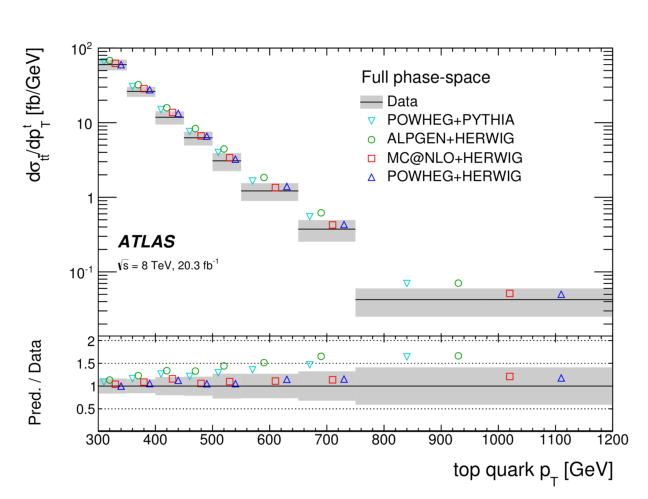
\includegraphics{boosted_top_pt.pdf}
  \caption{Section efficace différentielle des quarks tops en fonction
    de l'impulsion transverse mesurée par l'expérience ATLAS dans les
    collisions proton-proton à 8~TeV. Figure tirée de la
    référence~\cite{atlas_collaboration_measurement_2015}}
  \label{fig:boosted_top_pt}
\end{figure}

\subsection{Quarks top et supersymétrie}
\label{sec:top:boosted:susy}

Comme mentionné dans la section~\ref{sec:susy:mssm:sparticules}, les
partenaires supersymétriques des quarks de troisième génération ainsi
que le gluino doivent avoir une masse de l'ordre du TeV pour que le
problème de la hiérarchie des masses soit réglé dans le MSSM.  Dans
plusieurs réalisation du MSSM ayant ces propriétés, le mode de
désintégration en top + $\tilde{\chi}_1^0$ est parmi les modes
dominants pour le stop et le sbottom. Les particules supersymétriques
étant produites en paires, il y a possibilité de créer une paire de
quarks top lors de production directe de stops et sbottoms. De plus,
si les masses des squarks de première et deuxième générations sont
plus élevées que la masse du gluino, alors ce dernier désintègre
préférablement en une paire $\tilde{t}$ ou $\tilde{b}$ +
$\tilde{\chi}_1^0$ si les masses des stops et des sbottoms sont plus
petites que la sienne ou en un triplet top + top + $\tilde{\chi}_1^0$
via un stop/sbottom virtuel sinon.  Lors de production de paires de
gluinos, il peut donc y avoir jusqu'à quatre quarks tops dans l'état
final. Les masses du gluino, du stop et du sbottom sont au moins de
l'ordre du TeV donc beaucoup plus grande que celle du top, ce qui lui
permet d'acquérir une grande impulsion
transverse~\cite{bandyopadhyay_boosted_2011}.

Puisque la production de paires $t\overline{t}$ a une grande
section efficace au LHC et représente un bruit de fond important pour
plusieurs recherches de nouvelles
physique~\cite{atlas_collaboration_measurement_2015}, l'identification
efficace des quarks tops est d'une importance primordiale pour, par
exemple, discriminer les événements $t\overline{t}$ de productions de
paires de gluinos~\cite{ATLAS-CONF-2015-067}.

\section{Les variables de sous-structure}
\label{sec:top:sous_structure}

Il est possible de tirer avantage du chevauchement entre les gerbes de
0.4~mm originant des quarks tops et se désintégrant hadroniquement en
reconstruisant les gerbes avec un grand rayon ($>0.8$~mm). Il est
ensuite possible d'analyser les structures présentes dans ces grandes
gerbes pour identifier les tops. Le travail consiste à identifier des
\emph{variables de sous-structures} qui capturent les différences
entre les gerbes originant de quarks top et celles originant de gluons
ou de quarks légers. La variable de sous-structure la plus simple, la
masse de la gerbe, sera présentée dans la
section~\ref{sec:top:sous_structure:masse}. Une variable un peu plus
complexe, la \emph{N-subjetiness}, sera quant à elle traitée dans la
section~\ref{sec:top:sous_structure:tau_ij}.

\subsection{Masse}
\label{sec:top:sous_structure:masse}

La reconstruction d'une gerbe à partir des données enregistrées par
ATLAS commence par la formation de grappes contiguës en trois
dimensions de cellules de calorimètres activées au-dessus d'un certain
seuil. Ces grappes, auxquelles sont associée une quadri-impulsion de
masse nulle, sont ensuite regroupées en gerbes dans un certain rayon
qui est un paramètre de l'algorithme de regroupement. Lors des
simulations Monte Carlo, les constituants sont plutôt les
quadri-impulsions avec masse des particules générées. Une masse peut
alors être associée à la gerbe en fonction de l'énergie et de
l'impulsion des grappes constituantes:
\begin{equation}
  m_{gerbe} = \left(\sum_iE_i\right)^2 - \left(\sum_i\overrightarrow{p}\right)^2
\end{equation}

Les gerbes originant des quarks top ont, en moyenne, une plus grande
masse que celles originant de quarks légers ou de
gluons~\cite{_boosted_2015} à cause de la masse importante du top, comme le montre la
figure~\ref{fig:mass_distr}.

\begin{figure}
  \centering
  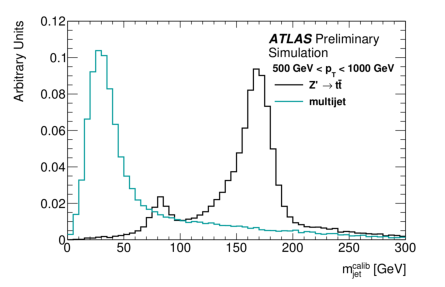
\includegraphics[width=.5\textwidth]{mass_distr.pdf}
  \caption{Distribution de la masse des gerbes pour un
    signal enrichi en quark tops ($Z' \rightarrow t\overline{t}$) et
    un bruit de fond riche en gluons et quarks légers. Les deux maxima
    de la distribution du signal correspondent aux masses du $W$ et du
    top. Figure tirée de la référence~\cite{_boosted_2015}.}
  \label{fig:mass_distr}
\end{figure}

% \subsection{Échelle de division}
% \label{sec:top:sous_structure:d_ij}

\subsection{N-subjetiness}
\label{sec:top:sous_structure:tau_ij}

La variable N-subjetiness, $\tau_N$, est une quantité qui caractérise
une gerbe comme contenant $N$ sous-gerbes. Pour calculer cette
variable, il faut d'abord regrouper les constituants~\footnote{grappes
  de cellules de calorimètre dans les données, particules dans les
  simulations} d'une gerbe en $N$ sous-gerbes de rayon plus petits que
la gerbe originale. Ensuite, $\tau_N$ est calculée comme étant la
somme pondéré par l'impulsion transverse de la distance entre chaque
constituant et la sous-gerbe la plus proche:
\begin{eqnarray}
  \tau_N = \frac{\sum_kp_T^{(k)}\ min\{\Delta R_{1,k},\Delta R_{2,k},\ldots,\Delta R_{N,k}\}}{\sum_kp_TR_0}
\end{eqnarray}

La valeur de $\tau_N$ est petite lorsque la plupart des constituants
sont alignés sur les $N$ sous-gerbes, indiquant que la gerbe est
constitué d'au plus $N$ sous-gerbes, et est grande lorsque plusieurs
constituants à haut $p_T$ ne sont pas dans une sous-gerbes, indiquant
que la gerbe est constitué de plus de $N$ sous-gerbes. Le quarks tops,
lorsqu'il se désintègre hadroniquement, engendre un quark $b$ et une
paire quarks-antiquarks. On s'attend donc à observer de petites
valeurs de $\tau_3$ pour de telles gerbes. De plus, les
désintégrations de quarks légers et de gluons reconstruits en grande
gerbes originent le plus souvent de la production de paire de gerbes
par interaction forte~\footnote{Communément appelé bruit de fond
  \emph{QCD dijet}} et ont donc de petites valeurs de
$\tau_2$~\cite{thaler_identifying_2011}.

En pratique, il est plus courant d'utiliser le ratio de ces deux
quantités, $\tau_{32}\equiv\tau_3/\tau_2$, qui permet de différencier
les gerbes originant de tops (trois sous-gerbes $\rightarrow$ petites
valeurs de $\tau_{32}$) de celles originant de paires de gerbes de
quarks légers ou de gluons (deux sous-gerbes, grandes valeurs de
$\tau_{32}$)~\cite{_boosted_2015}. La figure~\ref{fig:nsubj} montre le
pouvoir discriminatoire de cette variable.

\begin{figure}
  \centering
  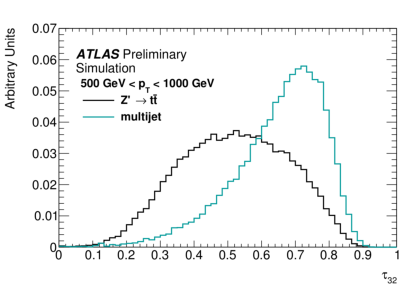
\includegraphics[width=.5\textwidth]{nsubj.pdf}
  \caption{Distributions de $\tau_{32}$ pour un signal enrichi en
    quark tops ($Z' \rightarrow t\overline{t}$) et un bruit de fond
    riche en gluons et quarks légers. Figure tirée de la
    référence~\cite{_boosted_2015}.}
  \label{fig:nsubj}
\end{figure}

\subsection{Performance}
\label{sec:top:sous_structure:perf}

Un discriminant basé due la masse de la gerbe et le ratio $\tau_{32}$
a été mis au point pour identifier les quarks tops dans les collisions
à 13~TeV enregistrée par le détecteur ATLAS en 2015. La
figure~\ref{fig:tagging} montre qu'on peut reconnaître $\approx 80\%$
des gerbes originant des tops tout en rejetant $\approx 80\%$ des
gerbes dues aux paires de quarks légers ou de gluons sur un grand
intervalle d'impulsion transverse~\cite{_boosted_2015}.

\begin{figure}[h]
  \centering
  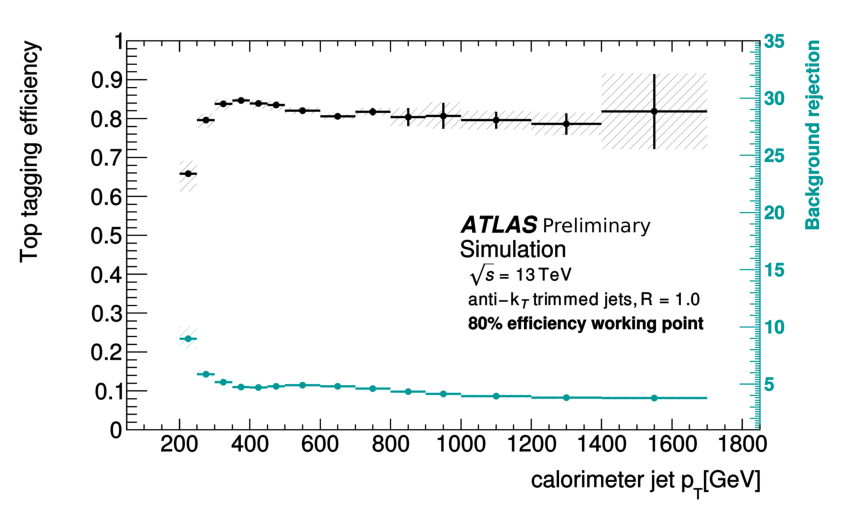
\includegraphics{tagging.pdf}
  \caption{Performance d'un discriminant basé due la masse de la gerbe
    et le ratio $\tau_{32}$ pour un signal enrichi en tops
    $(Z' \rightarrow t\overline{t})$ et un bruit de fond de paires de
    quarks léger ou de gluons. La mesure du rejet du bruit de fond est
    l'inverse du taux de faux positifs. Figure tirée de la
    référence~\cite{_boosted_2015}.}
\label{fig:tagging}
\end{figure}

% \section{Identification par apprentissage machine}
% \label{sec:top:ml}

% \subsection{Introduction à l'apprentissage machine}
% \label{sec:top:ml:intro}

% \subsection{Identification des quarks top}
% \label{sec:top:ml:top}

% \subsection{Identification des bosons W par apprentissage profond}
% \label{sec:top:ml:w}


%%% Local Variables:
%%% mode: latex
%%% TeX-master: "memoire"
%%% End:
